\documentclass[10pt]{article}

\usepackage{amsfonts, amsthm, fullpage, tikz}

\newcommand{\card}[1]{\left| #1 \right|}
\newcommand{\nat}{\mathbb{N}}
\newcommand{\ints}{\mathbb{Z}}
\newcommand{\reals}{\mathbb{R}}
\newcommand{\chtitle}[1]{\noindent \vspace{5mm}\textbf{Chapter #1}\vspace{3mm}}
\newcommand{\images}{/home/gparker/classes/341/images}

\begin{document}
\begin{flushleft}
\textbf{Geoffrey Parker - grp352 \\
CS 341 Automata Theory \\
Homework 3 \\
Due Thursday, Jan. 31}
\end{flushleft}
This assignment covers Sections 5.1 -- 5.6. \\

\begin{enumerate}
\addtocounter{enumi}{1}
% ---
% 2
% ---

\item
Show a DFSM to accept each of the following languages:
\begin{enumerate}

\addtocounter{enumii}{1}
% b
\item
$\{w \in \{a, b\}^* : w$ does not end in $ba\}$.
\begin{proof}[Answer:] $ $\\
\begin{flushleft}
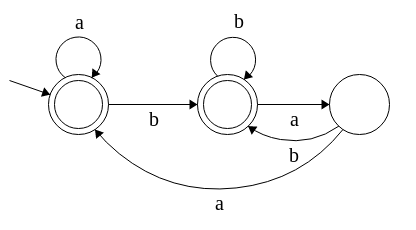
\includegraphics[scale=.5]{\images /hw3fsm2bsolution.png}
\end{flushleft}
\end{proof}


% c
\item
$\{w \in \{0, 1\}^* : 2$ corresponds to the binary encoding, without leading $0$'s, of natural numbers that are evenly divisible by $4\}$.
\begin{proof}[Answer:] $ $\\
\begin{flushleft}
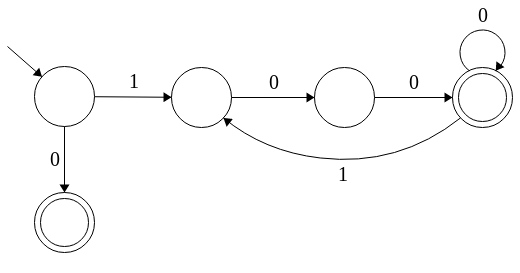
\includegraphics[scale=.5]{\images /hw3fsm2csolution.png}
\end{flushleft}
\end{proof}

\pagebreak
% d
\item
$\{w \in \{0, 1\}^* : 2$ corresponds to the binary encoding, without leading $0$'s, of natural numbers that are powers of $4\}$.
\begin{proof}[Answer:] $ $\\
\begin{flushleft}
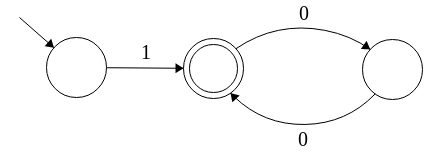
\includegraphics[scale=.45]{\images /hw3fsm2dsolution.png}
\end{flushleft}
\end{proof}

\addtocounter{enumii}{2}
% g
\item
$\{w \in \{0, 1\}^* : w$ does not have $001$ as a substring $\}.$
\begin{proof}[Answer:] $ $\\
\begin{flushleft}
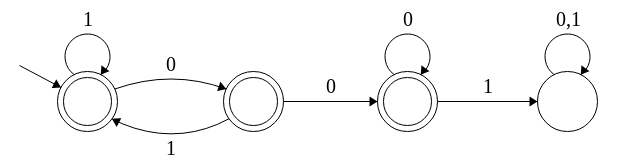
\includegraphics[scale=.45]{\images /hw3fsm2gsolution.png}
\end{flushleft}
\end{proof}

\addtocounter{enumii}{4}
% l
\item
The set of binary strings with at most one pair of consecutive $0$'s and at most one pair of consecutive $1$'s.
\begin{proof}[Answer:] $ $\\
\begin{flushleft}
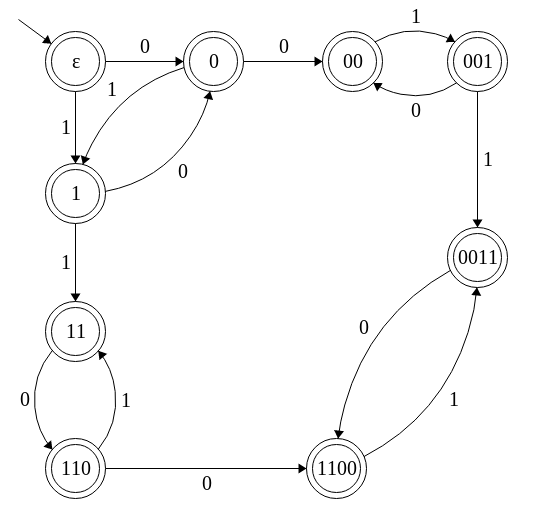
\includegraphics[scale=.45]{\images /hw3fsm2lsolution.png}
\end{flushleft}
\end{proof}
\end{enumerate}

% ---
% 3
% ---

\item
Consider the children's game Rock, Paper, Scissors.  We'll say that the first player to win two rounds wins the game.  Call the two players $A$ and $B$.
\begin{enumerate}

%a
\item
Define an alphabet $\Sigma$ and describe a technique for encoding Rock, Paper, Scissors games as strings over $\Sigma$. (Hint: each symbol in $\Sigma$ should correspond to an ordered pair that describes the simultaneous actions of $A$ and $B$.)
\begin{proof}[Answer:]
Let $\Sigma = \{ab\#cd : a,b,c,d \in \{R, P, S\}\}$.  Let $R$ stand for Rock, $P$ for Paper, and $S$ for Scissors.  Let $a$ and $b$ represent the actions of $A$ and $B$ in round 1, and $c$ and $d$ their actions in round 2.
\end{proof}

%b
\item
Let $L_{RPS}$ be the language of Rock, Paper, Scissors games, encoded as strings as described in part (a), that correspond to wins for player $A$.  Show a DFSM that accepts $L_{RPS}$.
\begin{proof}[Answer:] $ $\\
\begin{flushleft}
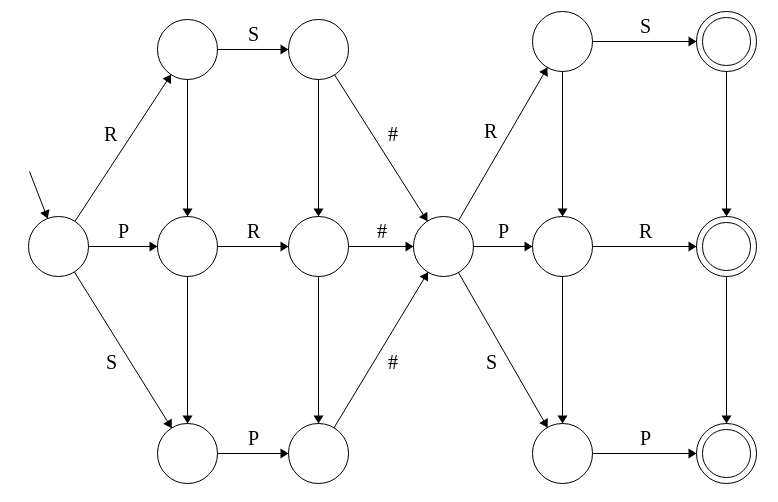
\includegraphics[scale=.45]{\images /hw3fsm3bsolution.png}
\end{flushleft}
\end{proof}
\end{enumerate}

% ---
% 4
% ---

\item
If $M$ is a DFSM and $\epsilon \in L(M)$, what simple property must be true of $M$?
\begin{proof}[Answer:]
The start state of $M$ must be accepting.
\end{proof}

\pagebreak
% ---
% 5
% ---

\item
Consider the following NDFSM M: \\

\begin{center}
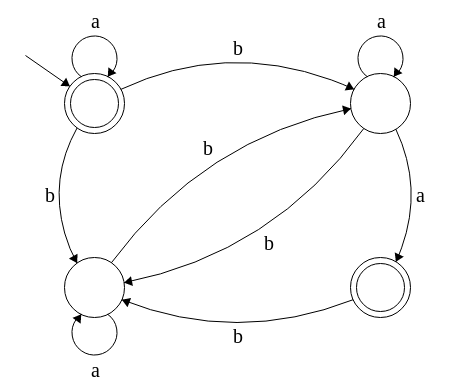
\includegraphics[scale=.5]{\images /hw3fsm5.png}
\end{center}

For each of the following strings $w$, determine whether $w \in L(M)$:
\begin{enumerate}
%a
\item
$aabbba$.
\begin{proof}[Answer:]
Yes.
\end{proof}

%b
\item
$bab$.
\begin{proof}[Answer:]
No.
\end{proof}

%c
\item
$baba$.
\begin{proof}[Answer:]
Yes.
\end{proof}
\end{enumerate}

\pagebreak
% -
% 6
% -

\item
Show a possibly nondeterministic FSM to accept each of the following languages:
\begin{enumerate}

%a
\item
$\{a^nba^m : n, m \geq 0, n \equiv _3 m\}$.
\begin{proof}[Answer:] $ $\\
\begin{flushleft}
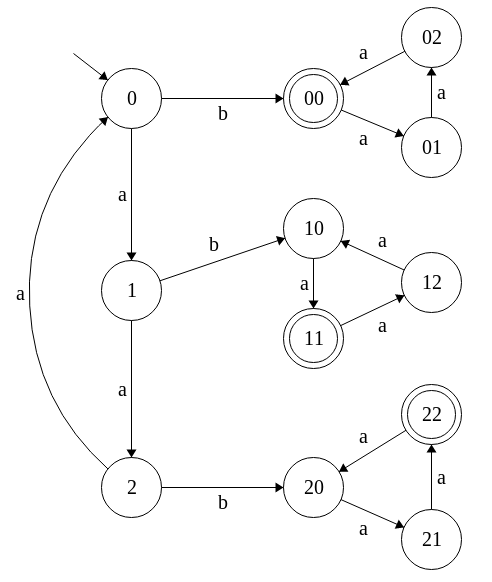
\includegraphics[scale=.45]{\images /hw3fsm6asolution.png}
\end{flushleft}
\end{proof}

%b
\item
$\{w \in \{0, 1\}^* : w$ contains both $101$ and $010$ as substrings\}.
\begin{proof}[Answer:] $ $\\
\begin{flushleft}
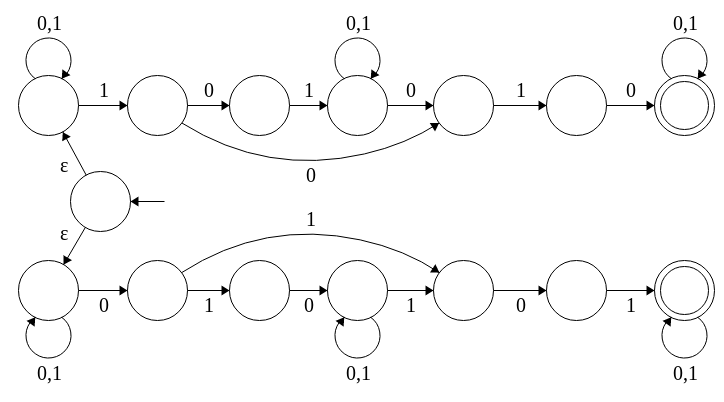
\includegraphics[scale=.45]{\images /hw3fsm6bsolution.png}
\end{flushleft}
\end{proof}
\end{enumerate}

\addtocounter{enumi}{2}
% ---
% 9
% ---

\item
Consider the following NDFSM. Use $ndfsmtodfsm$ to construct an equivilant DFSM.  Begin by showing the value of $eps(q)$ for each state $q$.

\begin{center}
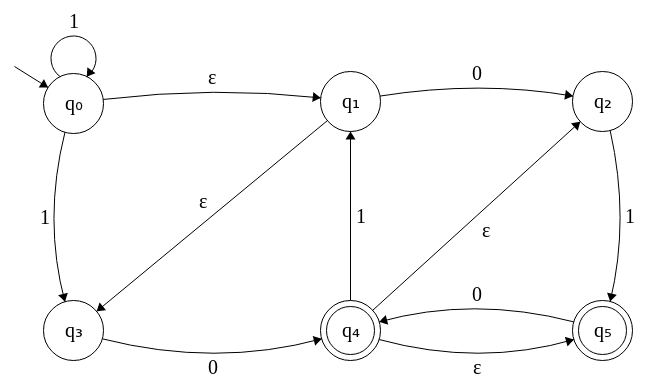
\includegraphics[scale=.5]{\images /hw3fsm9.png}
\end{center}

\begin{proof}[Answer:]$ $\\
\begin{description}
\item[] $eps(q_0) = \{q_0,\ q_1,\ q_3\}$
\item[] $eps(q_1) = \{q_1,\ q_3\}$
\item[] $eps(q_2) = \{q_2\}$
\item[] $eps(q_3) = \{q_3\}$ 
\item[] $eps(q_4) = \{q_2,\ q_4,\ q_5\}$
\item[] $eps(q_5) = \{q_5\}$
\end{description}
Start State: $s = \{q_0,\ q_1,\ q_3\}$ \\
State transitions: \\
\begin{description}
\item[] $\delta (\{q_0,\ q_1,\ q_3\},\ 0) = \{q_2,\ q_4,\ q_5\}$
\item[] $\delta (\{q_0,\ q_1,\ q_3\},\ 1) = \{q_0,\ q_1,\ q_3\}$
\item[]
\item[] $\delta (\{q_2,\ q_4,\ q_5\},\ 0) = \{q_2,\ q_4,\ q_5\}$
\item[] $\delta (\{q_2,\ q_4,\ q_5\},\ 1) = \{q_1,\ q_3,\ q_5\}$
\item[]
\item[] $\delta (\{q_1,\ q_3,\ q_5\},\ 0) = \{q_2,\ q_4,\ q_5\}$
\item[] $\delta (\{q_1,\ q_3,\ q_5\},\ 1) = \emptyset$
\end{description}
States $K = \{\{q_0,\ q_1,\ q_3\}, \{q_2,\ q_4,\ q_5\}, \{q_1,\ q_3,\ q_5\}\}$ \\
Accepting states $A = \{\{q_2,\ q_4,\ q_5\}, \{q_1,\ q_3,\ q_5\}\}$ \\
Let $\emptyset$ represent the dead state. \\ \\
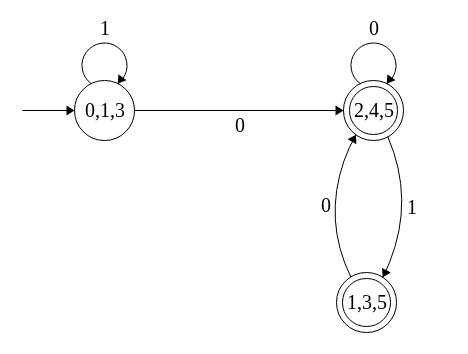
\includegraphics[scale=.5]{\images /hw3fsm9solution.png}
\end{proof}
\end{enumerate}
\end{document}
